\title{Week Five Assigment}
\author{Modal Models and Theorems of K}
\date{Due August 7, 5pm}
\documentclass{article}
\usepackage{fullpage}

\makeatletter
\let\Title\@title
\let\Author\@author
\makeatother

%\usepackage{amssymb}
\usepackage{amsmath}
\usepackage{mdwlist}
\usepackage[compact]{titlesec}
%\usepackage{graphicx}
%\usepackage[geometry,weather,misc,clock]{ifsym}
\usepackage{array}
%\usepackage{hanging}
\usepackage{hyphenat}
%\usepackage{epsfig}
%\usepackage{egame}
%\usepackage{booktabs}
\usepackage{nicefrac}
%\usepackage{bm}
\usepackage{multicol}

 \usepackage{tikz-qtree}
 \usepackage{markdown}
 \usepackage{prooftrees}

%\usepackage[pagebackref]{hyperref}
%\hypersetup{colorlinks=true,linkcolor=black,citecolor=black}
%\usepackage{etoolbox}
%\makeatletter
%\patchcmd{\BR@backref}{\newblock}{\newblock(Page~}{}{}
%\patchcmd{\BR@backref}{\par}{)\par}{}{}
%\makeatother


\usepackage{needspace}
\usepackage{textcomp}
%\usepackage{substr}
%\usepackage{natbib}
%\usepackage{nicefrac}
\usepackage{enumitem}
\setlist{noitemsep}
\usepackage{multirow}
%\usepackage{hyphenat}
\usepackage{tabulary}
\usepackage{booktabs}

%\renewcommand{\phi}{$\varphi$}
%\newcommand{\SP}{$S ^\prime$}
%\DeclareMathAlphabet{\mathpzc}{OT1}{pzc}{m}{it}
%\newcommand{\eqm}{equilibrium}
%\newcommand{\Eqm}{Equilibrium}
%\newcommand{\NE}{Nash Equilibrium}
%\newcommand{\NEs}{Nash Equilibria}
%\newcommand{\sth}{$^{\text{th}}$}
%\newcommand{\snd}{$^{\text{nd}}$}
%\newcommand{\sst}{$^{\text{st}}$}
%\newcommand{\ol}[1]{$\langle #1 \rangle$}
%\usepackage{pict2e}
%\usepackage{color}
%\usepackage{cclicenses}


%\usepackage[log-declarations=false]{xparse}


%\renewcommand{\labelitemi}{$\bullet$}

%\usepackage[garamond]{mathdesign}
\usepackage[no-math]{fontspec}
\setmainfont[Ligatures=TeX, BoldFont = Minion Pro Semibold]{Minion Pro}
%\setmainfont[Mapping=tex-text, BoldFont = Baskerville SemiBold]{Baskerville}
\usepackage[defaultmathsizes,italic]{mathastext}

\usepackage{fancyhdr}
\fancypagestyle{plain}{\renewcommand{\headrulewidth}{0pt} \fancyhf{}}
\pagestyle{plain}

%\DeclareSymbolFont{symbolsC}{U}{txsyc}{m}{n}
%\DeclareMathSymbol{\boxright}{\mathrel}{symbolsC}{128}
%\DeclareMathAlphabet{\mathpzc}{OT1}{pzc}{m}{it}


\setlength{\parindent}{0cm}

\usepackage{tikz}
%\usepackage{amsmath, amssymb}
\usetikzlibrary{positioning,arrows,calc}

\tikzset{
  modal/.style={>=stealth',
    shorten >=1pt,
    shorten <=1pt,
    auto,
    node distance=1.5cm,
    label distance=2pt,
    semithick},
  every label/.style={phantom,align=left},
  world/.style = {circle,draw,minimum size=0.5cm,fill=gray!15},
  modal every node/.style={world},
  point/.style={circle,draw,inner sep=0.5mm,fill=black},
  phantom/.style={rectangle,inner sep=0pt,draw=none,fill=none},
  reflexive above/.style={->,loop,looseness=7,in=60,out=120},
  reflexive below/.style={->,loop,looseness=7,in=240,out=300},
  reflexive left/.style={->,loop,looseness=7,in=150,out=210},
  reflexive right/.style={->,loop,looseness=7,in=30,out=330}
}

\newcommand{\mTrue}[1]{\ensuremath{#1}}
\newcommand{\mFalse}[1]{\ensuremath{\neg #1}}



\begin{document}
\maketitle
%\begin{center}\LARGE
%Final Exam
%\par\vskip 0.5em
%\large Philosophy 443
%\par\vskip 0.5em
%\large Time Allowed: 90 minutes \par\end{center}
%\vskip 1em












\begin{center}

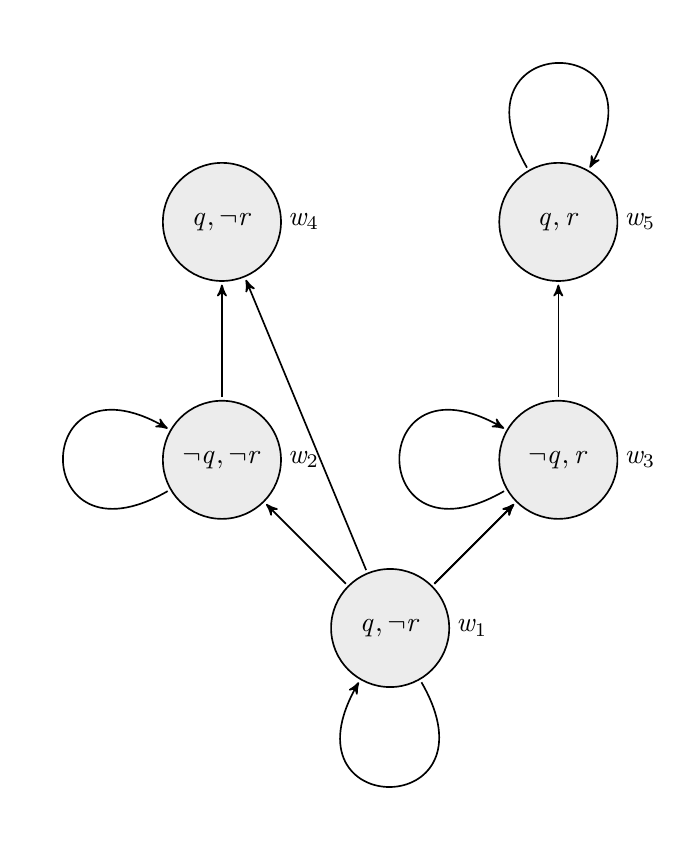
\begin{tikzpicture}[modal,world/.append style={minimum size=1.5cm}]
      \node[world] (w1) [label=right:$w_1$]{$q, \neg r$}; 
      \node[world] (w2) [label=right:$w_2$, above left=of w1]{$\neg q, \neg r$}; 
      \node[world] (w3) [label=right:$w_3$, above right=of w1] {$\neg q, r$};
      \node[world] (w4) [label=right:$w_4$, above =of w2] {$q, \neg r$};
      \node[world] (w5) [label=right:$w_5$, above =of w3] {$q, r$};
      \draw[->] (w1) to (w2);
      \draw[->] (w1) to (w3);
      \draw[->] (w1) to (w3);
      \draw[->] (w1) to (w4);
      \draw[->] (w2) to (w4);
      \draw[->] (w3) to (w5);
	  \path[->] (w1) edge[reflexive below] (w1);
	  \path[->] (w2) edge[reflexive left] (w2);
	  \path[->] (w3) edge[reflexive left] (w3);
	  \path[->] (w5) edge[reflexive above] (w5);
    \end{tikzpicture}
\end{center}
All questions concern the model above. It has five worlds, with accessibility relations show. The truth values for $q$ and $r$ at each world are shown within the within the worlds. (So at $w_1$, for example, $q$ is true and $r$ false.) Your task is to say which worlds $p$ must be true in order for some things to apply. You should make $p$ true at as few worlds as possible. If the question said ``Make $q \rightarrow p$ true everywhere in the model, the answer would be $w_1, w_4$ and $w_5$. You'll be marked incorrect if you also make $p$ true at $w_2$, even though that would indeed make $q \rightarrow p$ true.

\begin{enumerate}
\item Make $\Box p$ true at $w_1$
\item Make $\Box \Box p$ true at $w_1$
\item Make $\Diamond q \rightarrow p$ true everywhere in the model.
\item Make $\Box p \rightarrow p$ true everywhere in the model.
\item Make $\Diamond r \rightarrow p$ true everywhere in the model.
\item Make $\Box r \rightarrow p$ true everywhere in the model.
\item Make $\Diamond \Box r \rightarrow p$ true everywhere in the model.
\item Make $\Box (q \vee p)$ true everywhere in the model.
\item Make $\Box (q \rightarrow p)$ true everywhere in the model.
\item Make $\Box (r \vee p)$ true everywhere in the model.
\end{enumerate}

\newpage

\section*{The Logic K}
Which of these are theorems of K?

\begin{enumerate*}
\setcounter{enumi}{10}
\item $(\Box A \vee \Box B) \rightarrow \Box(A \vee B)$
\item $(\Box A \wedge \Diamond B) \rightarrow \Diamond(A \wedge B)$
\item $\Box (A \wedge \Diamond B) \rightarrow \Diamond(A \wedge B)$
\item $(\Box A \rightarrow \Box B) \rightarrow (\Diamond A \rightarrow \Diamond B)$
\item $\Box (A \rightarrow B) \rightarrow (\Diamond A \rightarrow \Diamond B)$
\end{enumerate*}

\end{document}